\documentclass{article}
\usepackage[utf8]{inputenc}
\usepackage{graphicx}
\usepackage{float}
\usepackage[numbers]{natbib}

\title{Projeto de Doutorado}
\author{Carlos Miguel Moreira Gonçalves}

\begin{document}

\maketitle

\section{Resumo}

\newpage

\section{Introdução}

%//! Introdução ao tema!


A escalada da urbanização \cite{urbanization} em tempos recentes desencadeou uma série de investimentos significativos na expansão e melhoria das ruas e avenidas, visando facilitar a locomoção nas cidades. Tais investimentos, caracterizados por aportes financeiros substanciais e extensos períodos dedicados à infraestrutura e finalização das obras, refletem o esforço para acompanhar as demandas de uma população em crescimento, como ilustrado na evolução da urbanização em Fortaleza na Figura \ref{fig:urbanizacao}. No entanto, a ausência de uma análise meticulosa da infraestrutura viária pode acarretar uma série de consequências adversas, incluindo a proliferação de congestionamentos, o aumento do nível de estresse entre motoristas e passageiros \cite{Hegewald2020}, a elevação do risco de acidentes e, consequentemente, um incremento nas emissões de gases nocivos ao meio ambiente \citep{Wang2018}. Esses efeitos colaterais não apenas comprometem a eficácia dos investimentos em mobilidade urbana, mas também impactam negativamente a qualidade de vida nas cidades.

\begin{figure}[H]
    \centering
    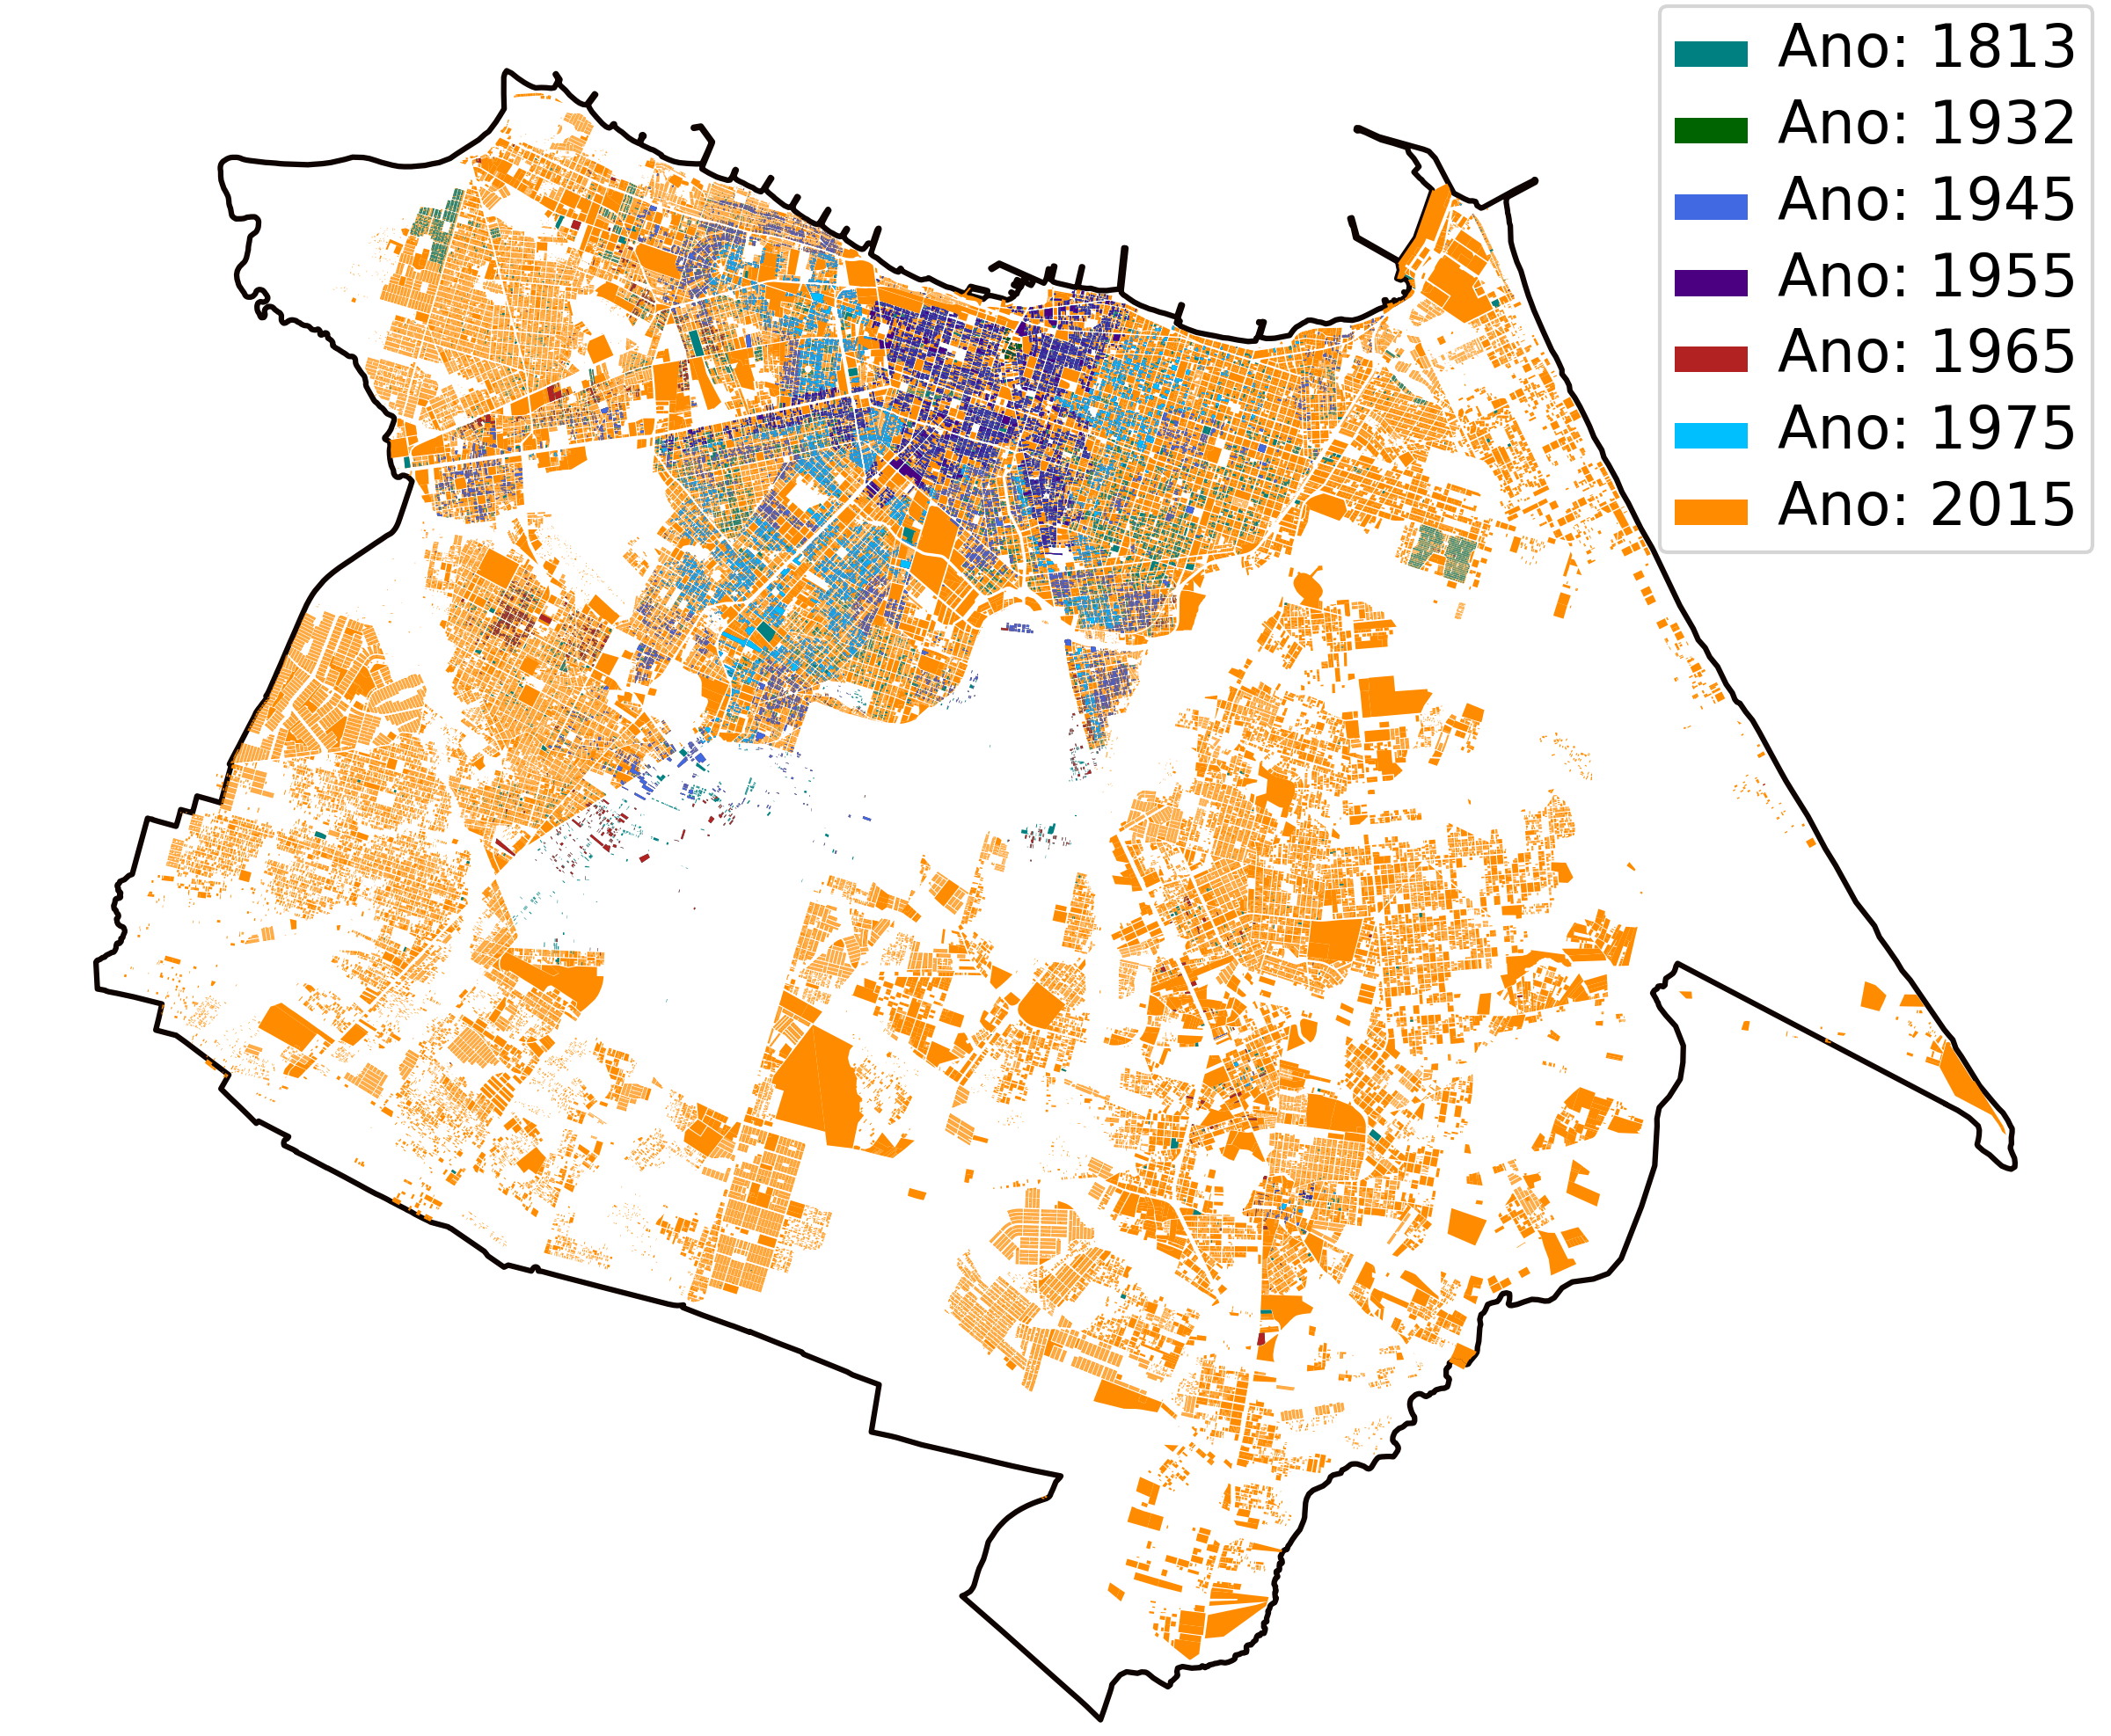
\includegraphics[width=0.7\textwidth]{img/urbanizacao.png}
    \caption{Evolução temporal da urbanização na cidade de Fortaleza.}
    \label{fig:urbanizacao}
\end{figure}

%//! Explicação da abordagem computacional!

Neste contexto, a modelagem computacional é uma ferramenta viável para abordar esses desafios urbanos complexos. Através de simulações precisas, é possível antecipar os impactos decorrentes de intervenções na infraestrutura viária, como a construção de novas vias, melhorias em rotas existentes, ou as consequências de obstruções temporárias provocadas por eventos climáticos adversos ou acidentes. O interesse por esta questão também se origina na presença de fundamentos físicos intrínsecos, tais como a lei da conservação do fluxo e o princípio de minimização de uma função de custo associada, além da manifestação de fenômenos críticos caracterizados por transições de fase entre estados de fluxo livre e congestionamento. 

%//! Explicação da transição de fase

Transições de fase representam transformações fundamentais que ocorrem em vários contextos, desde fenômenos físicos, como a mudança de estados da matéria, até aplicações em processos biológicos e a dinâmica de atribuição de tráfego, onde sistemas experimentam mudanças abruptas de estado. Essas mudanças abruptas são quantificáveis através de expoentes críticos, os quais não dependem da dimensionalidade do sistema. Essa independência dimensional sugere que problemas distintos, quando compartilham expoentes críticos similares, podem ser agrupados em uma categoria comum denominada classe de universalidade. 
\citet{Li2014,Zeng2018} exploraram a dinâmica do tráfego na rede viária de Pequim, revelando uma transição de fase. Eles criaram um parâmetro que determina a capacidade de uma via para acomodar o fluxo de veículos. Descobriram que há um valor crítico, que varia com o tempo, no qual emerge o fenômeno da percolação.

No entanto, a aplicação desta metodologia enfrenta obstáculos intrínsecos. Em primeiro lugar, a determinação das variáveis que um indivíduo considera ao escolher um percurso dentro do tecido urbano permanece incerta; não está claro se, ou como, as pessoas buscam otimizar seus trajetos em termos de tempo, custo ou conforto. Em segundo lugar, a velocidade de fluxo nas vias urbanas é diretamente influenciada pela densidade de tráfego, tornando a previsão do tempo de percurso uma questão dinâmica, sujeita a flutuações constantes em função do volume de veículos e por último a quantidade de dados disponíveis.

%//! Explicação da otimização do motorista

Assim como a corrente elétrica naturalmente encontra o caminho de menor resistência numa rede de resistores, e o fluido se desloca através do caminho de menor impedância em um meio poroso, seguindo a Lei de Darcy \citep{darcy}, os motoristas em uma rede urbana também buscam otimizar seus percursos. No entanto, ao contrário dos sistemas físicos regidos por leis bem definidas, o processo de decisão dos motoristas incorpora uma complexidade substancialmente maior. Esta complexidade deriva da diversidade de fatores que podem influenciar a escolha de uma rota, que vão além do mero cálculo de eficiência temporal ou de deslocamento. A seleção de um caminho pode ser afetada por aspectos como congestionamento, conhecimento da área, preferências pessoais, e até condições momentâneas, como o estado do tempo ou o humor do motorista resultando em trajetórias significativamente distintas daquelas focadas no benefício individual, ou uma abordagem altruísta, voltada para o bem-estar coletivo da sociedade. 

\citet{Anarchy} estudaram a razão do tempo considerando a otimização egoísta pelo tempo otimizando a sociedade e como esse valor se comporta em diferentes cidades e em modelos tradicionais de redes. 

%//! Coleta de dados

Por fim, a obtenção dos dados, apresenta desafios significativos em termos de sensibilidade temporal, uma vez que as condições de tráfego são altamente dinâmicas e sujeitas a variações diárias, sazonais e devido a eventos não regulares. Além disso, há questões morais intrínsecas à coleta e ao uso desses dados, particularmente no que se refere à privacidade dos indivíduos. As informações de localização e padrões de movimento, por exemplo, podem revelar detalhes sobre a vida das pessoas, levantando preocupações éticas sobre como esses dados são coletados, armazenados e utilizados. \citet{Simini2012} utilizaram um modelo para tentar estimar ,dado uma conexão entre cidades dos Estados Unidos, o número de pessoas que trafegam entre as duas cidades.

%//! Proposta do trabalho 

\newpage
\section{Objetivos}

Este projeto pretende estudar o problema de \textit{Traffic Assignment} a partir de simulações computacionais com foco em estudar a estrutura da rede e o seu comportamento perante mudanças na rede como a adesão de novas 

\newpage

\section{Métodos}

\newpage

\section{Resultados Esperados e Cronograma}

\newpage

\bibliographystyle{unsrtnat} % Use o estilo unsrtnat
\bibliography{reference.bib}

\end{document}
